\section{Shared behavior: a dictionary between the clocks and nonlinear dynamics}
\label{sec:dictionary}
\label{sec:tools}

With the clocks written as maps, the next question is which behaviors of nonlinear systems they show. Table~\ref{tab:dictionary} answers it for fifteen concepts at once, and it serves as the map of this section. Each row is a concept from nonlinear dynamics and each column is a clock. A cell names the observed behavior that the concept describes on that clock and marks its evidence level: \statusP\ when the correspondence is proved for a model of the system, \statusM\ when it has been measured in trained networks, and \statusC\ when it is a conjecture. A question mark means that we found no work that tests the concept on that clock.

\begin{figure}[t]
\centering
\resizebox{\textwidth}{!}{%
\begin{tikzpicture}[>=Stealth, font=\small,
  mass/.style={draw, thick, fill=blue!10, minimum width=9mm, minimum height=9mm},
  spring/.style={decorate, decoration={zigzag, amplitude=1.6mm, segment length=2.2mm, pre length=2mm, post length=2mm}, thick},
  ground/.style={pattern=north east lines, draw=none}]
% ---------------- (a) Duffing oscillator
\begin{scope}[shift={(0,0)}]
\node[anchor=west, font=\small\bfseries] at (-0.2,2.55) {(a) Duffing oscillator $\leftrightarrow$ generation regimes};
\fill[ground] (-0.15,0.2) rectangle (0,1.8); \draw[thick] (0,0.2) -- (0,1.8);
\node[mass] (m) at (3.0,1.0) {$M$};
\draw[spring] (0,1.35) -- node[above=1.2mm, font=\scriptsize] {$k_1,\ k_3$} ($(m.west)+(0,0.35)$);
\draw[thick] (0,0.65) -- (1.0,0.65); \draw[thick] (1.0,0.47) -- (1.0,0.83); \draw[thick] (1.0,0.47) -- (1.7,0.47) (1.0,0.83) -- (1.7,0.83);
\draw[thick] (1.4,0.53) -- (1.4,0.77); \draw[thick] (1.4,0.65) -- ($(m.west)+(0,-0.35)$); \node[font=\scriptsize] at (1.35,0.25) {$\zeta$};
\draw[->, thick, red!70!black] (m.east) -- ++(0.9,0) node[right, font=\scriptsize, align=left] {$A\cos\Omega\tau$\\$+\sqrt{2\zeta D}\,\xi(\tau)$};
\draw[->] (3.0,1.65) -- ++(0.6,0) node[above, font=\scriptsize] {$q$};
\node[anchor=west, font=\footnotesize] at (-0.2,-0.25) {$M\ddot q+\zeta\dot q+k_1q+k_3q^3=A\cos\Omega\tau+\sqrt{2\zeta D}\,\xi(\tau)$};
\node[anchor=west, font=\scriptsize, text=blue!50!black, align=left] at (-0.2,-0.75) {$k_1<0<k_3$: two wells. Language model: a well is a loop,\\the noise is the sampling temperature (Fig.~\ref{fig:atlas}).};
% language-model twin: the sampler feeds its output back
\begin{scope}[shift={(7.0,0.15)}]
\node[draw, thick, fill=orange!12, rounded corners=2pt, minimum width=1.7cm, minimum height=1.0cm, font=\scriptsize, align=center] (tf) at (0.9,1.35) {transformer\\$\mathrm{softmax}(z/T)$};
\node[draw, fill=orange!35, rounded corners=1pt, font=\scriptsize, minimum height=0.42cm] (yn) at (0.9,0.05) {$y_{n+1}$};
\draw[->, thick] (tf.south) -- node[right, font=\tiny] {sample} (yn.north);
\draw[->, thick, orange!70!black] (yn.east) -- ++(0.55,0) |- node[pos=0.25, right, font=\tiny, align=left] {appended\\to context} (tf.east);
\end{scope}
\end{scope}
% ---------------- (b) particle in a well
\begin{scope}[shift={(9.0,0)}]
\node[anchor=west, font=\small\bfseries] at (-0.2,2.55) {(b) Particle in a well $\leftrightarrow$ repetition loop};
\draw[thick, domain=-1.55:1.55, samples=60, smooth] plot ({1.15*\x+1.8}, {0.9*(\x*\x-1)*(\x*\x-1)+0.25});
\fill[blue!60!black] (0.65,0.36) circle (1.4mm);
\draw[<->, red!70!black] (1.8,0.25) -- (1.8,1.15) node[midway, right, font=\scriptsize] {$\Delta U$};
\draw[dotted] (0.65,0.25) -- (1.8,0.25);
\foreach \a in {30,90,150,210,270,330}{\draw[->, gray, thin] (0.65,0.36) -- ++(\a:0.35);}
\node[anchor=west, font=\footnotesize] at (-0.2,-0.25) {$\zeta\dot q=-U'(q)+\sqrt{2\zeta D}\,\xi(\tau)$,\quad rate $\propto e^{-\Delta U/D}$};
\node[anchor=west, font=\scriptsize, text=blue!50!black, align=left] at (-0.2,-0.75) {Language model: leaving a loop, $\Delta U\leftrightarrow$ logit gap $\Delta$,\\$D\leftrightarrow T$, exact by the softmax (Prop.~\ref{prop:arrhenius}, Fig.~\ref{fig:pair_escape}).};
% language-model twin: a repetition loop with exits
\begin{scope}[shift={(5.6,0.85)}]
\foreach \i/\ang in {1/90,2/0,3/270,4/180}{\node[circle, draw, fill=blue!8, inner sep=0pt, minimum size=4.6mm, font=\tiny] (b\i) at (\ang:0.62) {$a_{\i}$};}
\foreach \i/\j in {1/2,2/3,3/4,4/1}{\draw[->, blue!60!black] (b\i) to[bend left=30] (b\j);}
\node[circle, draw=gray, fill=gray!10, inner sep=0pt, minimum size=4.2mm, font=\tiny, text=gray] (ex) at (1.55,0.75) {$y$};
\draw[->, dashed, red!70!black] (b2) -- node[right, pos=0.35, font=\tiny, text=red!70!black] {$e^{-\Delta/T}$} (ex);
\end{scope}
\end{scope}
% ---------------- (c) metronomes on a rolling board
\begin{scope}[shift={(0,-4.3)}]
\node[anchor=west, font=\small\bfseries] at (-0.2,2.55) {(c) Metronomes $\leftrightarrow$ tokens over depth};
\draw[thick, fill=brown!20] (0.3,0.55) rectangle (4.3,0.75);
\foreach \x in {0.8,3.8}{\draw[thick] (\x,0.4) circle (0.15);}
\fill[ground] (0,0.1) rectangle (4.6,0.25); \draw[thick] (0,0.25) -- (4.6,0.25);
\foreach \x/\ang in {1.1/12,2.3/-8,3.5/20}{
  \draw[thick, fill=gray!15] (\x-0.3,0.75) -- (\x+0.3,0.75) -- (\x+0.12,1.75) -- (\x-0.12,1.75) -- cycle;
  \draw[very thick, blue!60!black] (\x,0.9) -- ++(90+\ang:0.95); \fill[blue!60!black] (\x,0.9) ++(90+\ang:0.7) circle (0.06);}
\draw[<->, red!70!black] (1.2,0.47) -- (3.4,0.47); \node[font=\scriptsize, red!70!black] at (2.3,0.95) {};
\node[anchor=west, font=\footnotesize] at (-0.2,-0.25) {$\dot\psi_i=\omega_i+\frac{J}{n}\sum_j\sin(\psi_j-\psi_i)$};
\node[anchor=west, font=\scriptsize, text=blue!50!black, align=left] at (-0.2,-0.75) {Language model: tokens over depth, coupled by attention;\\on the circle attention is this equation with $\omega_i=0$ (Eq.~\ref{eq:attn_kuramoto}).};
% language-model twin: tokens on the circle, coupled by attention
\begin{scope}[shift={(6.0,0.95)}]
\draw[gray, thin] (0,0) circle (0.75);
\foreach \a in {20,35,50,160,175,250,270}{\fill[orange!80!black] (\a:0.75) circle (0.07);}
\foreach \a/\b/\w in {20/35/0.9,20/50/0.8,35/50/0.9,160/175/0.9,250/270/0.9,50/160/0.25,175/250/0.25,20/270/0.25}{\draw[orange!60!black, opacity=\w, line width=0.5pt] (\a:0.75) -- (\b:0.75);}
\node[font=\tiny, align=center] at (0,-1.05) {tokens on the sphere,\\coupled by attention};
\end{scope}
\end{scope}
% ---------------- (d) a well that deepens
\begin{scope}[shift={(9.0,-4.3)}]
\node[anchor=west, font=\small\bfseries] at (-0.2,2.55) {(d) Deepening well $\leftrightarrow$ loop that reinforces itself};
\draw[thick, gray, domain=-1.4:1.4, samples=50, smooth] plot ({1.1*\x+1.6}, {0.45*(\x*\x)+0.9});
\draw[thick, domain=-1.4:1.4, samples=50, smooth] plot ({1.1*\x+1.6}, {1.0*(\x*\x)+0.25});
\fill[blue!60!black] (1.6,0.39) circle (1.4mm);
\draw[->, red!70!black, thick] (3.35,1.65) -- (3.35,0.75) node[midway, right, font=\scriptsize, align=left] {depth grows\\with time spent};
\node[anchor=west, font=\footnotesize] at (-0.2,-0.25) {$\Delta_c=\Delta_\infty-(\Delta_\infty-\Delta_1)\,e^{-(c-1)/c_\ast}$};
\node[anchor=west, font=\scriptsize, text=blue!50!black, align=left] at (-0.2,-0.75) {Language model: the repeated text in the context deepens\\the loop; reduced model of Section~\ref{sec:reduced} (Fig.~\ref{fig:reduced}).};
% language-model twin: the repeated text deepens the well
\begin{scope}[shift={(5.1,0.25)}]
\foreach \c/\h in {0/0.25,1/0.6,2/0.85,3/0.95}{
  \foreach \k in {0,1,2}{\node[draw, fill=orange!15, minimum width=0.24cm, minimum height=0.26cm, inner sep=0pt, font=\tiny] at (0.85*\c+0.26*\k,0) {\pgfmathparse{{"A","B","C"}[\k]}\pgfmathresult};}
  \fill[red!60!black] (0.85*\c+0.12,0.3) rectangle (0.85*\c+0.42,0.3+\h);}
\node[font=\tiny, text=red!60!black] at (1.9,1.55) {gap $\Delta_c$ grows, then saturates};
\node[font=\tiny] at (1.4,-0.35) {cycles of the loop in the context};
\end{scope}
\end{scope}
\end{tikzpicture}}
\caption{Four physical systems and their language-model twins. In each panel the mechanical system (left, with its governing equation) and the language model (right) look nothing alike, yet they share the term of the governing equation that produces the behavior; Section~\ref{sec:reduced} derives each correspondence. (a) A mass $M$ on a spring with linear stiffness $k_1$ and cubic stiffness $k_3$, friction coefficient $\zeta$, harmonic forcing of amplitude $A$ and frequency $\Omega$, and white noise $\xi$ of intensity $D$; with $k_1<0$ the potential $\tfrac12k_1q^2+\tfrac14k_3q^4$ has two wells. (b) An overdamped particle in a potential well under thermal noise of intensity $D$, whose escape rate over the barrier $\Delta U$ is given by Kramers' formula \eqref{eq:kramers}. (c) Metronomes on a board that can roll, which synchronize through the small motion of the board; their phases follow the Kuramoto model \eqref{eq:kuramoto}. (d) A well whose depth grows with the time the particle has spent in it and then saturates.}
\label{fig:models}
\end{figure}


\begin{table}[p]
\centering
\scriptsize
\setlength{\tabcolsep}{3pt}
\renewcommand{\arraystretch}{1.25}
\begin{tabularx}{\textwidth}{>{\raggedright\arraybackslash}p{2.1cm} >{\raggedright\arraybackslash}X >{\raggedright\arraybackslash}X >{\raggedright\arraybackslash}X}
\toprule
\textbf{Concept} & \textbf{Clock 1: layer time $\ell$} & \textbf{Clock 2: training time $t$} & \textbf{Clock 3: generation time $n$} \\
\midrule
Fixed point & Tokens collapse to a cluster; rank collapse \statusP\ \citep{geshkovski2023mathematical,dong2021attention}. Massive activations nearly input independent \statusM\ \citep{sun2024massive} & Convergence to a minimum; neural collapse at the end of training \statusM\ \citep{papyan2020prevalence} & Period-one loops (one token repeated) as the simplest case of degenerate repetition \statusM\ \citep{holtzman2019curious} \\
Linear stability, Jacobian spectrum & Dynamical isometry; layer Jacobians of trained models \statusP/\statusM\ \citep{pennington2017resurrecting,fernando2026dynamics} & Sharpness vs.\ $2/\eta$ \statusM\ \citep{cohen2021gradient} & Derivative of the feedback map factorizes through $1/T$ \statusM\ \citep{jones2026chaos} \\
Finite-time Lyapunov exponent & Ridges in input space separate classes \statusM\ \citep{storm2023finitetime}; per-layer profile over training \statusM\ (Sec.~\ref{sec:exp1}) & Sensitivity of runs to minibatch noise early in training \statusM\ \citep{frankle2019linear} & Divergence of nearby generations \statusM\ \citep{jaca2026chaos,jones2026chaos} \\
Edge of chaos, criticality & Order-chaos transition at initialization sets trainable depth \statusP\ \citep{poole2016exponential,schoenholz2016deep} & Edge of stability \statusM\ \citep{cohen2021gradient} & Critical temperature with power-law text statistics \statusM\ \citep{nakaishi2024phase} \\
Limit cycle (periodic orbit) & \na & Period-2 orbits of GD \statusP\ \citep{chen2022edge}; SGD converges to cycles \statusP\ \citep{chaudhari2017stochastic} & Repetition loops \statusM\ \citep{xu2022learning}; paraphrase 2-cycles \statusM\ \citep{wang2025unveiling}; loops converge in hidden-state space \statusM\ (Exp.~3) \\
Period doubling, route to chaos & \na & Larger step sizes give period doubling and chaos in minimal models \statusP\ \citep{zhu2022edgeofstability,kong2020stochasticity}; period-2 orbit, then irregular oscillation, in a transformer \statusM\ (Exp.~2) & Feigenbaum scaling in embedding feedback \statusM\ \citep{jones2026chaos} \\
Fractal boundary & \na & Trainable vs.\ divergent hyperparameters \statusM\ \citep{sohldickstein2024boundary}; interleaved trainable and divergent step sizes \statusM\ (Exp.~2); fractal attractors of optimizers \statusM\ \citep{tuci2026generalization} & \na \\
Basin of attraction & Class regions bounded by FTLE ridges \statusM\ \citep{storm2023finitetime} & Which minimum is reached depends on step size and batch size \statusM\ \citep{jastrzebski2017three} & Prompts that do or do not fall into loops \statusC \\
Metastability, slow manifold & Multi-cluster states last exponentially long \statusP\ \citep{geshkovski2024dynamic} & Plateaus \statusP\ \citep{saxe2013exact}; slow phase of pretraining \statusM\ \citep{zhang2026stability,wen2024warmupstabledecay} & Long coherent stretches before drift \statusC \\
Saddle and ghost & \na & Saddles dominate \statusM\ \citep{dauphin2014identifying}; abrupt learning from a ghost \statusP\ \citep{dinc2025ghost} & \na \\
Phase transition & \na & Grokking \statusP/\statusM\ \citep{rubin2023grokking,power2022grokking}; induction heads \statusM\ \citep{olsson2022incontext} & Low-$T$ repetitive vs.\ high-$T$ incoherent phase \statusM\ \citep{nakaishi2024phase,arnold2024phase}; narrow coherent window between them, also in a reasoning model \statusM\ (Exp.~3) \\
Noise-driven (Kramers) escape & \na & Escape of SGD from minima \statusP\ \citep{xie2020diffusion,mori2021powerlaw} & Escape from repetition loops, logit gap as barrier \statusP/\statusM\ (Prop.~\ref{prop:arrhenius}, Exp.~3); locking temperature \statusP\ (Prop.~\ref{prop:tlock}), horizon-dependent in practice \statusM\ (Exp.~3) \\
Synchronization, consensus & Clustering as consensus; Kuramoto form \statusP\ \citep{geshkovski2023mathematical,li2026diverse}; synchronization by noise \statusP\ \citep{agazzi2026stochastic} & \na & Collective dynamics of interacting models \statusP\ \citep{krishnamurthy2026stochastic} \\
Koopman, linearization & Local linear description of each layer \statusM\ \citep{fernando2026dynamics} & Koopman-based training and pruning \statusM\ \citep{dogra2020optimizing,redman2021operator}; lazy regime \statusP\ \citep{jacot2018neural} & \na \\
Conservation law, symmetry & Gradient-flow structure of attention \statusP\ \citep{sander2021sinkformers} & Symmetries give conserved quantities that finite steps break \statusP\ \citep{kunin2020neural} & \na \\
\bottomrule
\end{tabularx}
\caption{The Three-Clock Dictionary. Each cell gives the behavior that a dynamical-systems concept describes on one clock, with its evidence level (\statusP: proved in a model; \statusM: measured in trained networks; \statusC: conjecture) and representative references. Question marks are cells for which we found no study; they define the open problems of Section~\ref{sec:open}.}
\label{tab:dictionary}
\end{table}

\paragraph{Reading the table.} Fixed points, stability and Lyapunov exponents have been used on all three clocks, although with different meanings: on clock~1 they describe a single finite trajectory, on clock~2 the long-run behavior of an optimizer, and on clock~3 a random process. Phase transitions and escape appear on clocks~2 and~3 but not on clock~1, where the number of steps is fixed and small, so there is no long-time limit in which a transition could be sharp. Even so, the metastability result of \citet{geshkovski2024dynamic} shows that finite-time transients on clock~1 can be analyzed with care. Clock~2 is the best covered column, because optimization theory has always been a theory of iterated maps. Clock~1 is covered mostly by results at initialization and by models with simplified attention. Clock~3 is the youngest column, and most of its entries date from 2024 or later.

The rest of this section goes through the rows that carry most of the evidence. Each subsection defines one concept, shows it in a mechanical system and in a language model side by side, and summarizes what is known on each clock. The order follows the way the concepts build on each other: the stability of a fixed point and its loss through period doubling (Section~\ref{sec:eos}), the basins that decide which state is reached and the slow transients near unstable states (Section~\ref{sec:transitions}), the synchronization of coupled units (Section~\ref{sec:particles}), escape from a well under noise (Section~\ref{sec:escape}), the ways to tell periodic, noisy and chaotic motion apart in a measured signal (Section~\ref{sec:regimes}), and the growth of small perturbations (Section~\ref{sec:edgechaos}). Figure~\ref{fig:models} shows the four physical systems that recur in this comparison next to their language-model counterparts. Section~\ref{sec:reduced} then explains why each pair behaves alike.

\subsection{Stability, period doubling and the edge of stability}
\label{sec:eos}

We start with the simplest question one can ask of an iterated map: does a fixed point attract nearby states, and what happens when it stops doing so?

\paragraph{Maps, fixed points and stability.} A discrete-time system is a map $u_{t+1}=F(u_t)$. A fixed point $u^\ast=F(u^\ast)$ is linearly stable if every eigenvalue of the Jacobian $\mathrm{D}F(u^\ast)$ lies inside the unit circle. The textbook case is the explicit Euler scheme for a stiff ordinary differential equation: integrating $\dot u=-\lambda u$ with step $\eta$ gives $u_{t+1}=(1-\eta\lambda)u_t$, which converges only if $\eta\lambda<2$ and otherwise oscillates with growing amplitude. Gradient descent with step size $\eta$ on a quadratic with Hessian eigenvalue $\lambda$ is the same map, and this one-line calculation is the origin of the threshold $2/\eta$ in the edge-of-stability literature discussed below.

\paragraph{Periodic orbits and bifurcations.} A period-$k$ orbit is a fixed point of $F^{k}$, and under a change of parameter such orbits can appear, disappear or exchange stability. In a period-doubling bifurcation an eigenvalue crosses $-1$ and a period-2 orbit is born. The logistic map $u_{t+1}=\mu u_t(1-u_t)$, introduced as a model of insect populations, passes through a cascade of such doublings to chaos as $\mu$ grows \citep{may1976simple}, and the ratio of successive bifurcation intervals tends to a universal constant, $4.669\ldots$, for every smooth one-humped map \citep{feigenbaum1978quantitative}. In a saddle-node bifurcation a pair of fixed points collides and disappears. Just past it the trajectory still slows down where the pair used to be (a ``ghost''), which produces long plateaus followed by fast jumps \citep{strogatz2018nonlinear,dinc2025ghost}. Gradient descent on a double-well loss $\mathcal{L}(u)=(u^2-1)^2/4$ already shows both behaviors as $\eta$ grows. The minimum loses stability at $\eta=1$, a doubling cascade follows, and near $\eta\approx1.6$ the chaotic iterate hops between the two wells.

\begin{figure}[t]
\centering
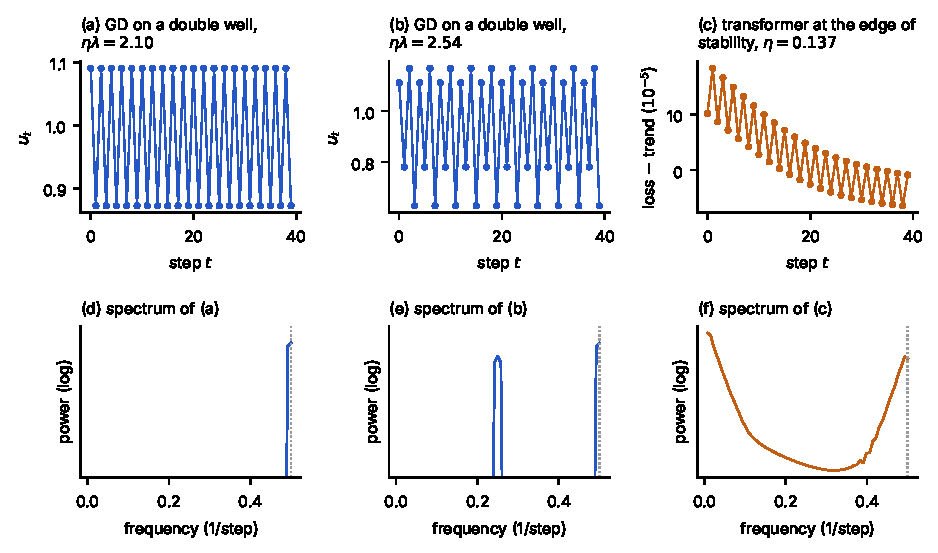
\includegraphics[width=\textwidth]{figs/pair_training.pdf}
\caption{Training as a dynamical system: period two at the edge of stability. (a, b) Gradient descent on the double well $\mathcal{L}(u)=(u^2-1)^2/4$, whose minimum has curvature $\lambda=2$, with $\eta\lambda=2.10$ and $2.54$: the last 40 iterates lie on a period-2 and a period-4 orbit. (d, e) Their power spectra, with peaks at frequencies $1/2$ and $1/4$. (c) The one-block transformer of Experiment~2 trained by full-batch gradient descent at $\eta=0.137$, at the edge of stability: training loss over the last 40 steps after removing a slow polynomial trend, in units of $10^{-5}$. The loss alternates from step to step. (f) Spectrum of the detrended loss over the last 400 steps: the same peak at $1/2$, on top of a low-frequency band from the slow modulation of the oscillation (Section~\ref{sec:exp2}).}
\label{fig:pair_training}
\end{figure}

\paragraph{On the clocks.} Classical optimization theory treats gradient descent as a discretization of gradient flow, which is valid when the step size is small compared with the inverse curvature. \citet{cohen2021gradient} showed that neural network training does not stay in that regime. Under full-batch gradient descent the sharpness, meaning the largest Hessian eigenvalue $\lambda_{\max}$, first rises (progressive sharpening) until it reaches $2/\eta$, and then hovers near that value while the loss keeps decreasing, though not monotonically. By the linear stability argument above, the iteration then sits on the boundary where the top direction loses stability. Adaptive methods show the same behavior with respect to the preconditioned sharpness \citep{cohen2022adaptive}.

For the regime as a whole there is now a continuous-time description. The central flow of \citet{cohen2024central}, an ODE for the time-averaged trajectory, keeps the sharpness at $2/\eta$ and predicts the loss curve of real networks, and \citet{berthier2026multiple} derive it by the method of multiple scales with three time scales. \citet{litman2026origin} shows that a weighted average of the curvature along the steps is forced to $2/\eta$. Bifurcation theory gives the local picture, with the onset of oscillation treated as a flip bifurcation near a manifold of minimizers (Appendix~\ref{app:related}). Section~\ref{sec:exp2} adds a measurement: in a small transformer the edge is multi-mode, with several eigenvalues above $2/\eta$, while the curvature along the step equals $2/\eta$.

At larger step sizes the map can become chaotic. Deterministic gradient descent on a multiscale objective, with a step size that resolves only the macroscopic scale, converges to a statistical distribution \citep{kong2020stochasticity}, and stochastic optimizers at the edge of stability have fractal attractors whose dimension has been related to generalization \citep{tuci2026generalization}. On clock~1 the corresponding question is whether a forward pass keeps signals at a constant size, which Section~\ref{sec:edgechaos} takes up, and on clock~3 it is the stability of a repetition loop, which Section~\ref{sec:escape} treats. Why training stays at the threshold instead of crossing it is explained with a reduced model in Section~\ref{sec:spring}, and Experiment~2 measures the whole sequence on a transformer.

\subsection{Basins, fractal boundaries and slow transients}
\label{sec:transitions}

A stable state is only useful if the system reaches it. Which state it reaches depends on where it starts, and on the way there it can linger near states that are not stable at all.

\paragraph{Basins and metastability.} The basin of attraction of an attractor is the set of initial conditions that reach it. Basin boundaries can be fractal \citep{mcdonald1985fractal}. In a periodically forced oscillator, such as a ship rolling in beam seas, the basin of safe motion around the upright state erodes into fractal fingers as the wave amplitude grows, so that capsizing becomes sensitive to the initial state well before the safe attractor itself disappears \citep{thompson1990fractal,thompson1997designing}. The set of trainable hyperparameters of a neural network has the same kind of boundary: \citet{sohldickstein2024boundary} found that the boundary between step sizes that train and those that diverge is fractal, in the same way as the boundary of bounded orbits of the quadratic map that defines the Mandelbrot set. Figure~\ref{fig:basins} shows both cases side by side. For a forced double-well oscillator the two basins are separated by a smooth curve at small forcing and by interleaved, fractal bands at larger forcing. For a small network trained by gradient descent with one step size per layer, the boundary between training and divergence keeps its jagged structure when magnified 25 times. A metastable state holds trajectories for a very long time without being an attractor, for example a cluster configuration of tokens that eventually merges \citep{geshkovski2024dynamic}.

\begin{figure}[t]
\centering
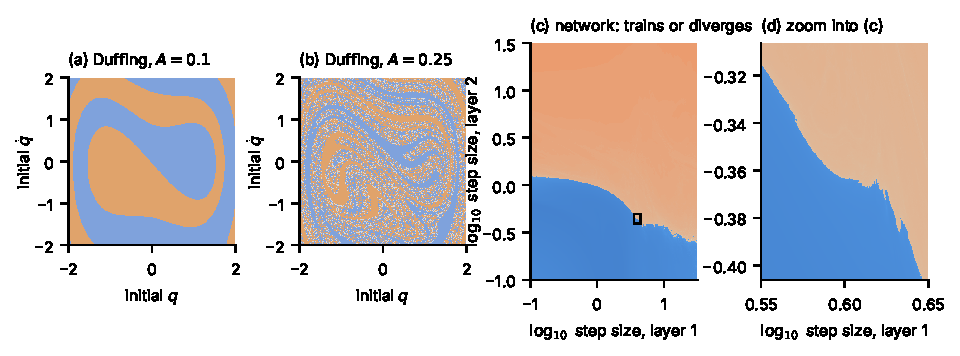
\includegraphics[width=\textwidth]{figs/basins.pdf}
\caption{Basins of attraction in a mechanical system and in training. (a, b) Forced double-well Duffing oscillator $\ddot q+0.25\dot q-q+q^3=A\cos(1.2\tau)$: the attractor reached from each initial condition after 40 forcing periods (blue: right well; orange: left well; gray: motion that keeps visiting both wells). At $A=0.1$ the basins are separated by a smooth boundary; at $A=0.25$ the boundary is fractal and a region of cross-well motion appears. (c) A one-hidden-layer tanh network (width 16) trained by full-batch gradient descent for 500 steps on eight random points, with separate step sizes for the two layers, following \citet{sohldickstein2024boundary}: blue runs train (darker: lower mean loss), orange runs diverge (lighter: later divergence). (d) Zoom into the box in (c).}
\label{fig:basins}
\end{figure}

\paragraph{Slow transients and abrupt transitions.} Near a saddle, or near the ghost of a fixed point that has just disappeared in a saddle-node bifurcation, a trajectory slows down for a long time and then moves on quickly. Training curves show both patterns. High-dimensional loss surfaces have far more saddles than local minima \citep{dauphin2014identifying}, and for deep linear networks the learning dynamics can be solved exactly: modes of the input-output map are learned one after another, separated by plateaus whose length depends on the initialization \citep{saxe2013exact}. In recurrent networks, abrupt learning after a long plateau has been traced to the ghost of a saddle-node bifurcation \citep{dinc2025ghost}.

Abrupt transitions in what a model can do are the clock-2 counterpart of a bifurcation. Grokking, where test accuracy jumps long after the training loss has saturated, was first reported on algorithmic data \citep{power2022grokking}; inside the network the change is gradual, with circuit-level measures that improve steadily before the jump \citep{nanda2023progress}, and a solvable two-layer model shows a first-order phase transition \citep{rubin2023grokking}. In language models, induction heads form during a short window of training, with a visible bump in the loss curve \citep{olsson2022incontext}, and across model scale abilities can appear suddenly \citep{wei2022emergent}, although part of the effect comes from discontinuous metrics \citep{schaeffer2023emergent}. Further explanations of these transitions are reviewed in Appendix~\ref{app:related}.

\subsection{Synchronization: tokens that cluster over depth}
\label{sec:particles}

Basins and transients concern a single trajectory. Clock~1 is organized instead by many tokens acting on each other, and the matching concept from dynamics is synchronization.

\paragraph{Synchronization and consensus.} Weakly coupled oscillators can lock their phases. \citet{bennett2002huygens} reconstructed Huygens' 1665 observation of this effect: two pendulum clocks hanging from a common beam end up swinging in antiphase, coupled through the small motion of the beam. Metronomes on a freely rolling board do the same \citep{pantaleone2002synchronization}, and tidal friction has locked the Moon's rotation to its orbit, so it always shows the Earth the same face \citep{goldreich1966spin}. The Kuramoto model reduces many such systems to phases $\psi_i$ with natural frequencies $\omega_i$ and coupling strength $J$,
\begin{equation}
\dot\psi_i=\omega_i+\frac{J}{n}\sum_{j=1}^{n}\sin(\psi_j-\psi_i),
\label{eq:kuramoto}
\end{equation}
and shows a transition to collective synchrony once $J$ exceeds a critical value set by the spread of the $\omega_i$ \citep{kuramoto1975self,acebron2005kuramoto}. Attention over depth has the same structure without the natural frequencies. Each token drifts toward a softmax-weighted average of the others, with weights $e^{\beta\langle x_i,x_j\rangle}$, so aligned tokens pull harder on each other \citep{geshkovski2023mathematical}. On the circle, with $x_i=(\cos\psi_i,\sin\psi_i)$, this gives $\dot\psi_i=Z_i^{-1}\sum_j e^{\beta\cos(\psi_j-\psi_i)}\sin(\psi_j-\psi_i)$, a Kuramoto model whose coupling depends on alignment \citep{li2026diverse}. With $\beta=0$ every token ends in one cluster; with large $\beta$ several clusters form and survive over a long stretch of depth before merging (Section~\ref{sec:kuramoto}).

\begin{figure}[t]
\centering
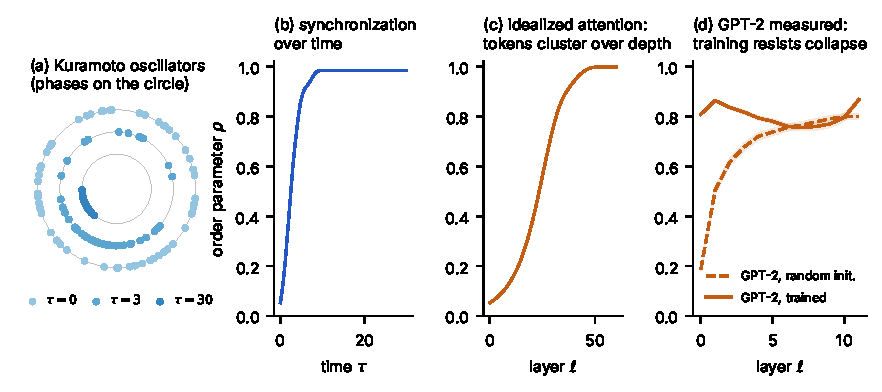
\includegraphics[width=\textwidth]{figs/pair_depth.pdf}
\caption{Depth as a dynamical system: synchronization of oscillators and clustering of tokens. (a) Kuramoto model \eqref{eq:kuramoto} with $n=60$, $J=1.5$ and $\omega_i\sim\mathcal N(0,0.3^2)$: phases at $\tau=0$, 3 and 30 (outer to inner ring). (b) Its order parameter $\rho=|n^{-1}\sum_j e^{\mathrm{i}\psi_j}|$. (c) The attention dynamics on the circle with $\beta=1$ and 60 tokens: the same order parameter, now over layers. (d) GPT-2, measured: order parameter of the residual stream entering each block, $\rho_\ell=\|n^{-1}\sum_i x_i^\ell/\|x_i^\ell\|\|$, for 20 prompts (mean $\pm$ one standard deviation). With random weights the tokens synchronize over depth as the idealized model predicts ($\rho$ from 0.19 to 0.80). The trained model starts from aligned embeddings ($\rho=0.81$) and stays between 0.76 and 0.87 over the twelve blocks.}
\label{fig:pair_depth}
\end{figure}

\paragraph{On clock 1.} The transformer differs from a plain residual network because the update of token $i$ depends on all tokens. \citet{lu2019improving} read a transformer layer as a splitting scheme for a convection-diffusion equation of interacting particles. \citet{sander2021sinkformers} proved that attention with doubly stochastic (Sinkhorn) normalization is a Wasserstein gradient flow. \citet{geshkovski2023emergence,geshkovski2023mathematical} studied a model in which tokens live on the unit sphere (a stand-in for layer normalization) and follow
\begin{equation}
\dot x_i = \Pi_{x_i}\Big(\frac{1}{Z_i}\sum_{j} e^{\beta\langle W_Q x_i, W_K x_j\rangle} W_V x_j\Big),
\label{eq:particles}
\end{equation}
where $\Pi_x$ projects onto the tangent space, $W_Q,W_K,W_V$ are the query, key and value matrices, and $\beta$ acts as an inverse temperature. They proved that, for broad choices of $W_Q,W_K,W_V$, the tokens cluster as time (depth) grows, in the simplest cases to a single point. Clustering is the particle-system version of an older observation: stacks of pure attention lose rank doubly exponentially with depth \citep{dong2021attention}, and rank collapse at initialization slows training \citep{noci2022signal}. Similar results hold for oversmoothing in attention-based graph networks, which \citet{wu2023demystifying} analyze as nonlinear time-varying dynamical systems.

Real models have finite depth, so the long-time limit of \eqref{eq:particles} describes them only partly. \citet{geshkovski2024dynamic} proved that particles stay near a configuration of several clusters for an exponentially long time before they merge, and a stack of finite depth spends its layers inside such a long-lived transient.

\subsection{Noise-driven escape}
\label{sec:escape}
\label{sec:sgd}

Stable states and basins describe a system without noise. With noise, a system can leave a basin that it would never leave otherwise, and the time it takes is the subject of one of the oldest results of statistical physics.

\paragraph{Kramers' escape problem.} Add noise of intensity $D$ to a system resting at the bottom of a well of depth $\Delta U$. The mean time to leave the well grows as
\begin{equation}
\bar\tau\simeq\frac{2\pi}{\omega_{\mathrm{w}}\,\omega_{\mathrm{b}}}\,\zeta\,e^{\Delta U/D}
\label{eq:kramers}
\end{equation}
in the overdamped limit with friction coefficient $\zeta$, where $\omega_{\mathrm{w}}$ and $\omega_{\mathrm{b}}$ are set by the curvature at the bottom of the well and at the top of the barrier \citep{kramers1940brownian,hanggi1990reaction}. The exponential factor is the Arrhenius law for the rate of chemical reactions, with temperature in the role of $D$ \citep{arrhenius1889reaktionsgeschwindigkeit}. In engineering the same question decides whether a ship capsizes in random waves or a structure snaps through to a buckled state. Escape from potential wells under deterministic periodic forcing is a related problem, where the escape threshold in forcing amplitude depends on the forcing frequency and on the shape of the well \citep{farid2019escape,farid2022escape}. In mechanics escape is usually a failure to be avoided; in text generation the well is a repetition loop, and escape is what one wants. Figure~\ref{fig:escape_time} shows the two behaviors over time: a particle that rests in a well and hops, and GPT-2 sampled at a low temperature, which falls into repetition loops and leaves them.

\begin{figure}[t]
\centering
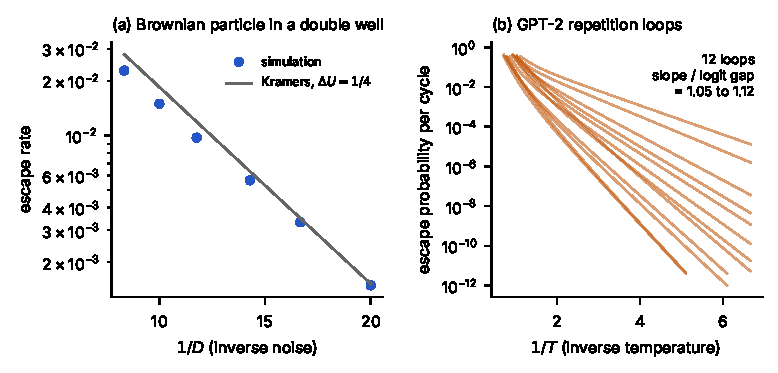
\includegraphics[width=0.8\textwidth]{figs/pair_escape.pdf}
\caption{Noise-driven escape in a mechanical system and in a language model, on the same axes. (a) An overdamped particle, $dq=-U'(q)\,d\tau+\sqrt{2D}\,d\mathcal{W}$, in the double well $U(q)=(q^2-1)^2/4$ with barrier $\Delta U=1/4$: inverse mean first-passage time from $q=-1$ to $q=+1$ (400 particles per noise level) against $1/D$, with Kramers' rate $(\sqrt2/2\pi)\,e^{-\Delta U/D}$. The fitted slope gives $\Delta U=0.23$. (b) Twelve repetition loops of GPT-2 from Experiment~3: exact probability of leaving the loop during one cycle, computed from the stored logits, against $1/T$. At low temperature each curve is a straight line whose slope is the logit gap of the loop, as Proposition~\ref{prop:arrhenius} predicts (ratio of slope to gap 1.05 to 1.12).}
\label{fig:pair_escape}
\end{figure}

\begin{figure}[t]
\centering
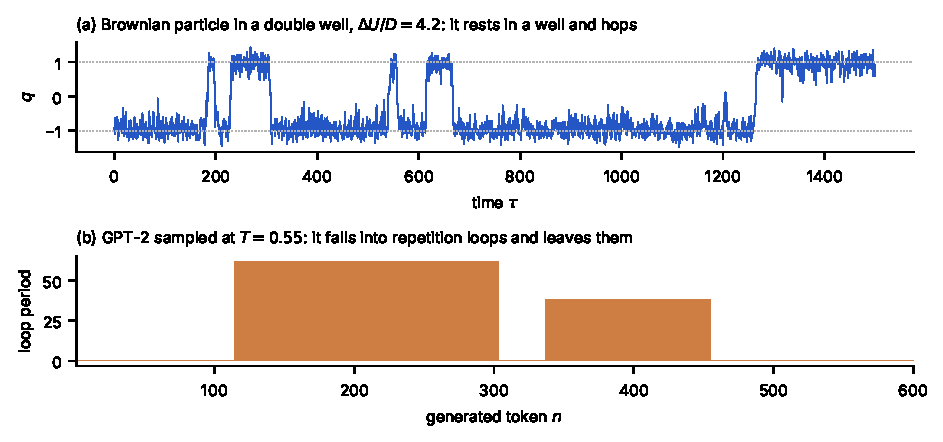
\includegraphics[width=\textwidth]{figs/escape_time.pdf}
\caption{Escape over time. (a) Position of an overdamped particle in the double well $U(q)=(q^2-1)^2/4$ under noise of intensity $D=0.06$: long rests near $q=\pm1$ separated by quick hops. (b) GPT-2 continuing one prompt with plain temperature sampling at $T=0.55$: at each generated token, the period of the repetition loop the text is in, where a stretch counts as a loop when it repeats at least three times (zero outside a loop). The text enters two loops, stays in each for more than a hundred tokens and leaves both.}
\label{fig:escape_time}
\end{figure}

\paragraph{On clock 2.} Minibatch noise turns clock~2 into a stochastic process. Stochastic modified equations approximate SGD with step size $\eta$ and batch size $B$ by the SDE
\begin{equation}
d\theta=-\nabla\mathcal{L}(\theta)\,dt+\sqrt{\tfrac{\eta}{B}\,C(\theta)}\;d\mathcal{W}_t ,
\label{eq:sme}
\end{equation}
where $C$ is the covariance of per-example gradients, $\mathcal{W}_t$ is a Wiener process, and time is measured in units of $\eta$ \citep{li2015stochastic}. Near a minimum with Hessian $H$ the drift is linear, the process is of Ornstein-Uhlenbeck type, and its stationary covariance $\Sigma$ solves the Lyapunov equation $H\Sigma+\Sigma H=(\eta/B)\,C$, so the ratio $\eta/B$ acts as a temperature \citep{mandt2017stochastic,smith2017bayesian,jastrzebski2017three}. Because SGD noise is anisotropic and state dependent, the stationary distribution is not a Gibbs distribution of the training loss, and the dynamics can converge to limit cycles instead of points \citep{chaudhari2017stochastic}.

Escape from a minimum is the most direct use of this theory. \citet{xie2020diffusion} derived a Kramers-type rate for SGD and found that, unlike isotropic Langevin dynamics, SGD favors flat minima exponentially in the ratio of barrier height to Hessian eigenvalues, and anisotropic noise aligned with the curvature helps escape from sharp minima \citep{zhu2018anisotropic}. Because the noise of SGD is multiplicative, the escape rate can instead scale as a power of the loss ratio between saddle and minimum \citep{mori2021powerlaw}, and heavy-tailed gradient noise points toward L\'evy-driven escape, dominated by single large jumps \citep{simsekli2019tailindex}. Which of these laws holds in language-model pretraining has not been measured.

\paragraph{On clock 3.} With greedy or low-temperature decoding, models fall into loops that repeat a phrase or sentence until the length limit \citep{holtzman2019curious}. At $T=0$ the chain is deterministic and the loop is one of its periodic orbits. \citet{xu2022learning} showed that loops reinforce themselves: the probability of repeating a sentence grows with the number of times it already appears in the context. Unlikelihood training \citep{welleck2019neural}, truncation rules \citep{hewitt2022truncation,meister2022locally} and feedback control of perplexity \citep{basu2020mirostat} can be read in part as attempts to keep the chain out of these attractors; \citet{fu2020theoretical} give a theoretical analysis of why they form. Recent work studies the inside of the loop: how it shows up in residual-stream dynamics before it becomes visible in the output \citep{zhang2026uncovering}, and the conditions under which a loop ``locks'' so that escape becomes impossible in practice under a given sampler \citep{chen2026repetition}. Loops also appear at the level of whole texts. Repeated paraphrasing converges to period-two attractor cycles even with sampling noise \citep{wang2025unveiling}. Reasoning models loop too, mostly at low temperature, which \citet{pipis2025wait} trace to errors in learning hard steps of a task and to temporally correlated errors.

Section~\ref{sec:loops} shows that for repetition loops the correspondence with Kramers' problem is an exact identity, and derives when a loop locks.

\subsection{Telling regimes apart from data}
\label{sec:regimes}

The previous subsections described the dynamics through models. In an experiment one usually has only a measured signal, and the same distinctions, between periodic motion, noise and chaos, must be read from it.

\paragraph{Four pictures of a signal.} An experimentalist who sees only a signal classifies the motion with four standard pictures. The time history shows the motion directly. In the power spectrum a periodic motion gives sharp peaks at its frequency and harmonics, and noise or chaos gives a broad band. In the phase portrait a periodic orbit is a closed curve and noise fills a region. The recurrence plot marks the pairs of times $(i,j)$ at which the state returns close to itself, $R_{ij}=1$ if $\|u_i-u_j\|<\epsilon_R$, and a periodic orbit draws long lines parallel to the diagonal \citep{eckmann1987recurrence}. Two numbers condense the last two pictures: the normalized entropy of the spectrum, $\mathcal{H}_s$, from 0 for a single line to 1 for white noise, and the determinism DET, the fraction of recurrent points that lie on diagonal lines \citep{marwan2007recurrence}. Figure~\ref{fig:atlas} applies the four pictures to a forced double-well Duffing oscillator at three noise levels and to GPT-2 at three sampling temperatures. In both systems the quiet regime is a periodic orbit (for GPT-2, a repetition loop), with sharp spectral peaks and diagonal recurrence lines, and DET falls as the noise or the temperature grows. Over 10 noise seeds and 10 prompts, the median DET is 0.97, 0.48 and 0.42 for the Duffing oscillator and 0.67, 0.32 and 0.17 for GPT-2, and the median $\mathcal{H}_s$ is 0.18, 0.60 and 0.90 against 0.70, 0.95 and 0.95. The analogy has a limit that the pictures make plain: the spectra of coherent and of incoherent text are both close to flat, so for GPT-2 these two regimes differ in their recurrence structure and in the level of surprisal, not in the spectrum. Recurrence analysis of hidden states has recently been applied to the reasoning traces of DeepSeek-R1-Distill \citep{pham2026mind}, and recurrence plots and correlation dimensions to chain-of-thought trajectories \citep{jaca2026chaos}.

\begin{figure}[t]
\centering
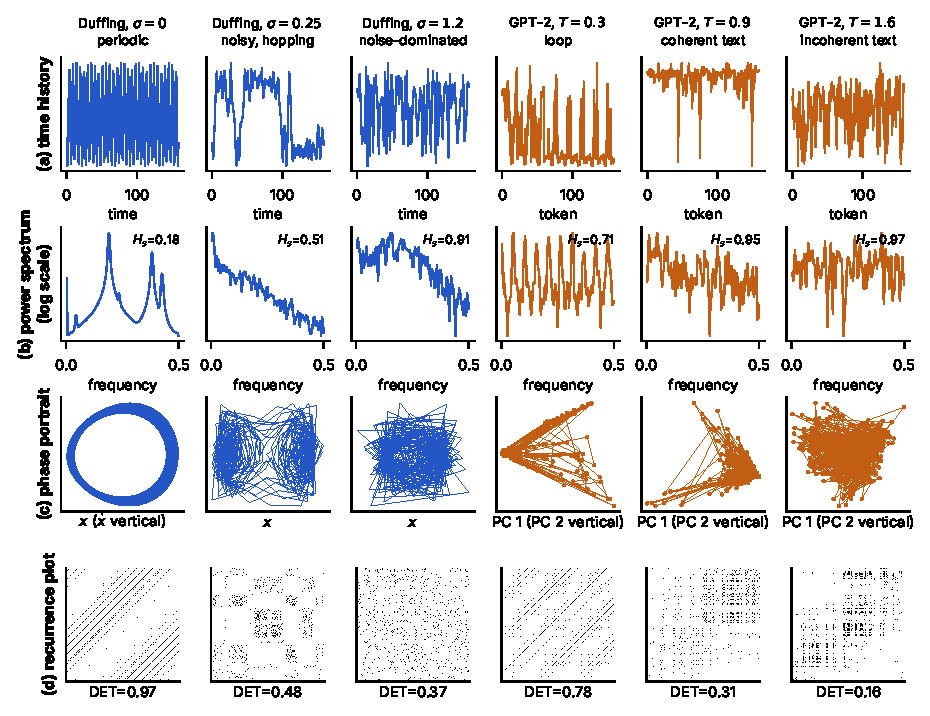
\includegraphics[width=\textwidth]{figs/atlas.pdf}
\caption{Generation as a dynamical system: the same four pictures for a mechanical oscillator and for a language model. Left: the forced double-well Duffing oscillator $\ddot q+0.25\dot q-q+q^3=0.1\cos(1.2\tau)+\sqrt{0.5D}\,\xi(\tau)$, sampled once per time unit, at noise intensities $D=0$ (periodic orbit in one well), $0.125$ (noisy orbits with hops between the wells) and $2.88$ (noise-dominated). Right: GPT-2 continuing one prompt for 576 tokens at $T=0.3$ (a loop of period 19), $0.9$ (coherent text) and $1.6$ (incoherent text); the state is the final hidden state of each token, scaled to unit norm and standardized per feature, after a transient of 64 tokens. (a) Time history of the first coordinate ($q$, or the first principal coordinate of the hidden state). (b) Its power spectrum (Welch), with the spectral entropy $\mathcal{H}_s$. (c) Phase portrait: $(q,\dot q)$, or the first two principal coordinates. (d) Recurrence plot of the full state at a fixed recurrence rate of 5\%, with the determinism DET.}
\label{fig:atlas}
\end{figure}

\paragraph{On clock 3.} At the level of statistics over many generations, temperature produces something close to a phase transition. \citet{nakaishi2024phase} varied $T$ in GPT-2 and found a low-temperature phase with repetitive structure, a high-temperature phase of incoherent text, and power-law correlations close to those of natural language at the transition point. Seen from clock~3, both phases are failures, and useful text lives in a window between them. The lower edge of the window is the loop escape of Section~\ref{sec:escape}. The upper edge, where sampling noise spreads over so much of the vocabulary that the text loses coherence, has no dynamical definition yet, and Experiment~3 locates it only through proxies. \citet{arnold2024phase} proposed statistical methods to detect such transitions automatically from output distributions. \citet{jones2026chaos} found that in the continuous feedback version of generation, temperature and activation steering move the system between periodic orbits and chaos with positive finite-time Lyapunov exponents, with period-doubling scaling and periodic orbits proved by interval arithmetic. In chain-of-thought trajectories, \citet{jaca2026chaos} report sensitive dependence on initial conditions together with bounded evolution and fractal structure in hidden-state space. Sorting many generated trajectories into regimes (fixed point, periodic, irregular) without labels is a response-regime identification problem, for which unsupervised data-driven methods exist in mechanics \citep{farid2024unsupervised}.

\subsection{Lyapunov exponents, order and chaos}
\label{sec:edgechaos}

The last concept measures how fast nearby trajectories separate. It is the quantity behind sensitivity to initial conditions, and it applies to all three clocks.

\paragraph{Lyapunov exponents.} For a trajectory $u_0,u_1,\dots$ the finite-time Lyapunov exponent over $K$ steps is
\begin{equation}
\Lambda_K(u_0) = \frac{1}{K}\log \sigma_{\max}\big(\mathrm{D}F(u_{K-1})\cdots \mathrm{D}F(u_0)\big),
\label{eq:ftle}
\end{equation}
where $\sigma_{\max}$ is the largest singular value. Positive values mean that nearby trajectories separate exponentially, so that a perturbation of size $\delta$ reaches size one after about $\log(1/\delta)/\Lambda_K$ steps. \citet{lorenz1963deterministic} found this sensitivity in a three-variable truncation of atmospheric convection, and it gives weather forecasts a finite horizon however accurate the initial data are. The limit $K\to\infty$, when it exists, is the largest Lyapunov exponent. Deep networks have a fixed and small number of steps, so only finite-time exponents make sense for clock~1 \citep{storm2023finitetime}.

\paragraph{On clock 1.} One line of work treats a randomly initialized deep network as a random dynamical system and asks whether small input differences grow or shrink with depth. \citet{poole2016exponential} found an order-to-chaos transition controlled by the weight and bias variances $\sigma_w^2,\sigma_b^2$. For a wide fully connected network with nonlinearity $\phi$, the correlation between two nearby inputs is multiplied at each layer by
\begin{equation}
\chi_1=\sigma_w^2\,\mathbb{E}\big[\phi'(\sqrt{Q^\ast}\,G)^2\big] ,
\label{eq:chi1}
\end{equation}
where $Q^\ast$ is the fixed point of the length map and $G$ is a standard Gaussian variable. Inputs converge for $\chi_1<1$ (order) and separate for $\chi_1>1$ (chaos), so $\ln\chi_1$ plays the role of a Lyapunov exponent per layer; \citet{schoenholz2016deep} showed that the depth over which signals propagate diverges at the transition, so networks are trainable to large depth only near it. The idea goes back to the chaotic phase of random recurrent networks \citep{sompolinsky1988chaos}. Requiring all singular values of the input-output Jacobian to be close to one (dynamical isometry) speeds up training further \citep{pennington2017resurrecting} and allowed 10{,}000-layer convolutional networks to train \citep{xiao2018dynamical}. For transformers, \citet{cowsik2024geometric} track the geometry of $n$ token representations as a discrete-time system of interacting particles and derive conditions on the initialization that make deep transformers trainable.

For trained networks, \citet{storm2023finitetime} computed finite-time Lyapunov exponents \eqref{eq:ftle} of fully connected classifiers and found ridges of large exponents in input space that separate the classes, much like coherent structures in fluid flows. Our first experiment (Section~\ref{sec:exp1}) applies the same quantity to the residual stream of language models across training.

\paragraph{What a dynamical model of depth must reproduce.} Interpretability research gives facts that any dynamical model of clock~1 has to reproduce. Predictions decoded from intermediate layers improve gradually, which suggests a trajectory that refines its estimate step by step \citep{belrose2023eliciting}. Deleting or swapping middle layers hurts much less than touching the first or last ones, consistent with distinct stages of the trajectory \citep{lad2024remarkable}. Token trajectories through depth stay close to a low-dimensional manifold \citep{sarfati2024lines}. A few activations are orders of magnitude larger than the rest and nearly independent of the input \citep{sun2024massive}, which together with attention sinks \citep{xiao2023efficient} can be read as a near fixed point of the depth dynamics. Experiment~1 measures how training changes the stretching along this trajectory.

\paragraph{On clock 3.} Training uses teacher forcing, while generation feeds the model its own outputs. Small errors therefore compound along clock~3, a problem known as exposure bias \citep{bengio2015scheduled,wang2020exposure}. Errors snowball in multi-step reasoning \citep{dziri2023faith} and in hallucinated justifications \citep{zhang2023language}, and next-token prediction can fail on planning tasks that require looking ahead \citep{bachmann2024pitfalls}. In dynamical terms these are statements about the growth of perturbations along a trajectory of the closed-loop system: if the finite-time exponent of clock~3 is positive, an early error of size $\delta$ grows roughly as $\delta\,e^{\Lambda_K K}$ over the next $K$ tokens. This exponent has not been measured for language models (\op{3}).

\paragraph{Koopman linearization.} Lyapunov exponents describe a nonlinear map through its linearization along one trajectory. A different, global linearization exists: a nonlinear map acts linearly on functions of the state, called observables, $h\mapsto h\circ F$ \citep{koopman1931hamiltonian}. Eigenfunctions of this Koopman operator give coordinates in which the dynamics is linear, and finite approximations can be learned from data \citep{mezic2005spectral}. Dynamic mode decomposition, for instance, extracts the oscillation frequencies and spatial modes of a jet in crossflow directly from snapshots \citep{rowley2009spectral}. Related data-driven methods learn linear embeddings of nonlinear dynamics with neural networks \citep{lusch2017deep} or sparse governing equations from data \citep{brunton2015discovering}. Koopman methods have also been applied to the training dynamics of neural networks \citep{dogra2020optimizing,redman2021operator}.
